% Drawing 154/05-6 -- folder 154, batch 05, archive page 96 (PDF page 97).
% Transcription: dessins en couleur : en haut à gauche, un disque traversé de pseudo-droites orange, avec, sur le bord, les points $u$, $u'$, $s$, $t$ et les arcs marqués $\alpha$, $\beta$, $\gamma$, chaque segment de bord entre eux marqué « $\frac12$ » par une accolade ; au centre, un petit disque traversé de pseudo-droites orange ; en haut à droite, un disque de même facture, avec $u$, $u'$, des arcs $\alpha$, $\beta$ très courts et un long arc $\gamma$ en bas, les segments de bord marqués « $\frac12$ » ; en bas, deux bandes horizontales (bords vert clair, axe orange) coupées de faisceaux de droites orange, les bords renforcés en noir par segments, en tirets ou pleins, qui se croisent au milieu en un point marqué $u$, $u'$ dans la seconde
% Kind: disks with boundary arcs marked 1/2; bands cut by pencils. Method 2 (schematic redraw from the facsimile). Status: partial.
% Notes: Top left: a disk crossed by orange pseudolines, with on the rim the points u, u', s, t and the arcs alpha, beta, gamma (thick black), each stretch of rim between them marked « 1/2 » by a brace. Centre: a small disk crossed by orange pseudolines. Top right: a disk of the same kind, with u, u', very short arcs alpha, beta and a long arc gamma at the bottom, the stretches of rim marked « 1/2 ». Bottom: two horizontal bands (light green borders, orange axis) cut by pencils of orange lines, the borders reinforced in black by segments, dashed or solid, crossing in the middle at a point marked u, u' in the second. Read from the page view; the strands in the disks and the black reinforcements of the bands are schematic. Still differs from the facsimile: Read from the page view; the strands in the disks and the black reinforcements of the bands are schematic.
% Coordinates: 1 unit = 1 mm = 1/100 of the crop width (bbox in page fractions: [0.13, 0.082, 0.782, 0.515]).
% Redrawn by Claude (claude-opus-5-5), issue #73, 2026-11-07; not checked by a human; not compiled (no TeX in the session).
% Revised by Claude (claude-opus-5-5) 2026-11-09 (issue #128) after Michel's check: vertices snapped to exact intersections (drawn points on their lines, meeting ends on the stroke they meet, near-concurrent lines through one computed point, curve ends on their rim); labels at \small as in folder 80 batch 3. Status: partial.
% Rights: reproduces part of the work -- behind RENDER_TRANSCRIPTS, never published by itself.
\documentclass[tikz,border=3pt]{standalone}
\usepackage{amsmath,amssymb}
\usetikzlibrary{patterns,arrows.meta}
\tikzset{Or/.style={orange!90!black}, Ye/.style={yellow!80!orange}, Lg/.style={green!60!black!70}, Dg/.style={green!45!black}, Br/.style={brown!80!black}, Rd/.style={red!85!black}, Bl/.style={blue!70!black}, Gy/.style={black!40}, pencil/.style={black!45}, struck/.style={black!35}, mark/.style={circle,draw,inner sep=1.3pt}, pt/.style={circle,fill,inner sep=0.9pt}, opt/.style={circle,draw,fill=white,inner sep=1.1pt}}
\begin{document}
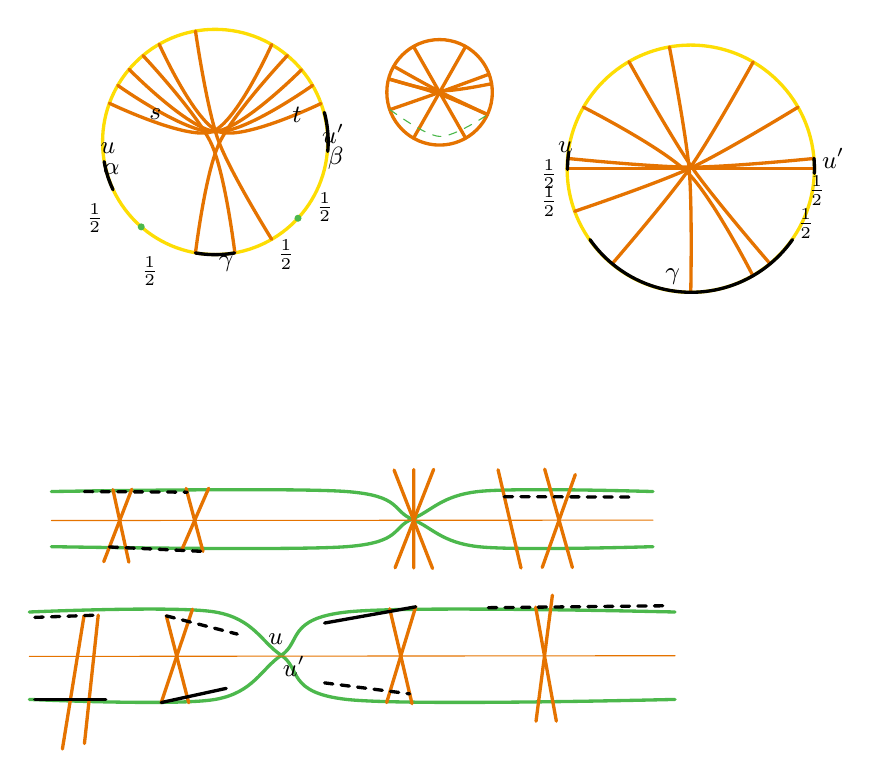
\begin{tikzpicture}[x=1mm,y=1mm,line cap=round,line join=round,font=\scriptsize]
\draw[Ye,very thick] (22.2,-16) circle[radius=14.3];
\draw[Or,very thick] plot[smooth, tension=0.55] coordinates {(8.77,-11.09) (21.8,-14.7) (29.38,-3.63)};
\draw[Or,very thick] plot[smooth, tension=0.55] coordinates {(35.64,-11.12) (22.7,-14.7) (15.09,-3.59)};
\draw[Or,very thick] plot[smooth, tension=0.55] coordinates {(9.83,-8.82) (22.1,-14.7) (33.17,-6.83)};
\draw[Or,very thick] plot[smooth, tension=0.55] coordinates {(34.57,-8.82) (22.3,-14.7) (11.27,-6.78)};
\draw[Or,very thick] plot[smooth, tension=0.55] coordinates {(13.03,-5.03) (21.7,-16.2) (24.7,-30.08)};
\draw[Or,very thick] plot[smooth, tension=0.55] coordinates {(31.37,-5.03) (22.7,-16.2) (19.7,-30.1)};
\draw[Or,very thick] plot[smooth, tension=0.55] coordinates {(19.7,-1.92) (22.6,-15.8) (29.38,-28.37)};
\draw[very thick] (8.1,-18.5) arc[start angle=190, end angle=205, x radius=14.3, y radius=14.3];
\draw[very thick] (36.5,-17.2) arc[start angle=-5, end angle=15, x radius=14.3, y radius=14.3];
\draw[very thick] (19.7,-30.1) arc[start angle=260, end angle=280, x radius=14.3, y radius=14.3];
\node[inner sep=1pt] at (8.6,-16.8) {\small $u$};
\node[inner sep=1pt] at (9,-19.4) {\small $\alpha$};
\node[inner sep=1pt] at (14.6,-12.5) {\small $s$};
\node[inner sep=1pt] at (32.6,-12.5) {\small $t$};
\node[inner sep=1pt] at (37.2,-15) {\small $u'$};
\node[inner sep=1pt] at (37.5,-18.1) {\small $\beta$};
\node[inner sep=1pt] at (23.6,-31.5) {\small $\gamma$};
\node[inner sep=1pt] at (6.9,-25.7) {\small $\frac12$};
\node[inner sep=1pt] at (13.9,-32.4) {\small $\frac12$};
\node[inner sep=1pt] at (31.2,-30.3) {\small $\frac12$};
\node[inner sep=1pt] at (36.1,-24.3) {\small $\frac12$};
\node[pt,Lg] at (12.81,-26.79) {};
\node[pt,Lg] at (32.72,-25.69) {};
\draw[Or,very thick] (50.7,-9.7) circle[radius=6.7];
\draw[Or,very thick] plot[smooth, tension=0.55] coordinates {(44.25,-8) (50.7,-9.5) (57.31,-8.6)};
\draw[Or,very thick] plot[smooth, tension=0.55] coordinates {(44.4,-11.9) (50.7,-9.7) (56.99,-7.4)};
\draw[Or,very thick] plot[smooth, tension=0.55] coordinates {(44.88,-6.39) (50.7,-9.6) (56.8,-12.53)};
\draw[Or,very thick] plot[smooth, tension=0.55] coordinates {(47.39,-3.88) (50.7,-9.7) (54.01,-15.52)};
\draw[Or,very thick] plot[smooth, tension=0.55] coordinates {(54.01,-3.88) (50.7,-9.7) (47.39,-15.52)};
\draw[Or,very thick] plot[smooth, tension=0.55] coordinates {(44.25,-8) (50.6,-9.9) (56.8,-12.53)};
\draw[Lg,dashed] plot[smooth, tension=0.55] coordinates {(44.4,-11.9) (50.7,-15.3) (56.8,-12.53)};
\draw[Ye,very thick] (82.6,-19.4) ellipse[x radius=15.7, y radius=15.7];
\draw[Or,very thick] plot[smooth, tension=0.55] coordinates {(67.01,-18.1) (82.6,-19.2) (98.25,-18.1)};
\draw[Or,very thick] plot[smooth, tension=0.55] coordinates {(66.9,-19.4) (82.6,-19.4) (98.3,-19.4)};
\draw[Or,very thick] plot[smooth, tension=0.55] coordinates {(68.98,-11.59) (82.2,-19.9) (90.5,-33)};
\draw[Or,very thick] plot[smooth, tension=0.55] coordinates {(79.89,-3.94) (82.4,-19.5) (82.6,-35.1)};
\draw[Or,very thick] plot[smooth, tension=0.55] coordinates {(90.53,-5.85) (82.5,-19.3) (72.6,-31.5)};
\draw[Or,very thick] plot[smooth, tension=0.55] coordinates {(96.22,-11.59) (82.6,-19.3) (67.86,-24.81)};
\draw[Or,very thick] plot[smooth, tension=0.55] coordinates {(74.75,-5.81) (82.8,-19.3) (92.68,-31.48)};
\draw[very thick] (69.8,-28.4) arc[start angle=215, end angle=325, x radius=15.7, y radius=15.7];
\draw[very thick] (67.1,-17.3) arc[start angle=172, end angle=180, x radius=15.7, y radius=15.7];
\draw[very thick] (98.3,-20) arc[start angle=-2, end angle=5, x radius=15.7, y radius=15.7];
\node[inner sep=1pt] at (66.7,-16.7) {\small $u$};
\node[inner sep=1pt] at (100.7,-18.1) {\small $u'$};
\node[inner sep=1pt] at (80.3,-33.1) {\small $\gamma$};
\node[inner sep=1pt] at (64.6,-20.1) {\small $\frac12$};
\node[inner sep=1pt] at (64.6,-23.6) {\small $\frac12$};
\node[inner sep=1pt] at (98.6,-22.2) {\small $\frac12$};
\node[inner sep=1pt] at (97.2,-26.4) {\small $\frac12$};
\draw[Lg,very thick] plot[smooth, tension=0.55] coordinates {(1.4,-60.4) (38.9,-60.4) (47.2,-63.9) (55.6,-67.4) (77.8,-67.4)};
\draw[Lg,very thick] plot[smooth, tension=0.55] coordinates {(1.4,-67.4) (38.9,-67.4) (47.2,-63.9) (55.6,-60.4) (77.8,-60.4)};
\draw[Or] (1.4,-64.08) -- (77.8,-64.03);
\draw[Or,very thick] (9.22,-60.16) -- (11.24,-69.37);
\draw[Or,very thick] (11.61,-60.11) -- (8.05,-69.31);
\draw[Or,very thick] (18.51,-60) -- (20.65,-68);
\draw[Or,very thick] (21.38,-59.98) -- (17.97,-67.79);
\draw[Or,very thick] (44.92,-57.67) -- (49.81,-70.17);
\draw[Or,very thick] (49.95,-57.58) -- (45.05,-70.08);
\draw[Or,very thick] (47.41,-57.6) -- (47.42,-70.1);
\draw[Or,very thick] (58.13,-57.64) -- (61.04,-70.11);
\draw[Or,very thick] (64.05,-57.56) -- (67.57,-70.05);
\draw[Or,very thick] (67.94,-58.24) -- (63.74,-70.04);
\draw[very thick,dashed] (5.6,-60.4) -- (18.64,-60.48);
\draw[very thick,dashed] (8.77,-67.44) -- (20.65,-68);
\draw[very thick,dashed] (58.92,-61.05) -- (75,-61.1);
\draw[Lg,very thick] plot[smooth, tension=0.55] coordinates {(-1.4,-75.7) (22.2,-75.7) (30.6,-81.2) (38.9,-86.8) (80.6,-86.8)};
\draw[Lg,very thick] plot[smooth, tension=0.55] coordinates {(-1.4,-86.8) (22.2,-86.8) (30.6,-81.2) (38.9,-75.7) (80.6,-75.7)};
\draw[Or] (-1.4,-81.34) -- (80.6,-81.25);
\draw[Or,very thick] (5.55,-76.15) -- (2.8,-93.1);
\draw[Or,very thick] (7.35,-76.09) -- (5.6,-92.4);
\draw[Or,very thick] (16,-76.19) -- (18.84,-87.22);
\draw[Or,very thick] (19.32,-75.34) -- (15.35,-87.2);
\draw[Or,very thick] (44.37,-75.29) -- (47.2,-87.34);
\draw[Or,very thick] (47.67,-75.04) -- (43.98,-87.2);
\draw[Or,very thick] (62.9,-75.08) -- (65.53,-89.56);
\draw[Or,very thick] (65.03,-73.56) -- (62.95,-89.57);
\draw[very thick,dashed] (-0.7,-76.38) -- (7.35,-76.09);
\draw[very thick] (-0.7,-86.8) -- (8.3,-86.8);
\draw[very thick,dashed] (16,-76.19) -- (25,-78.5);
\draw[very thick,dashed] (36.1,-84.7) -- (46.9,-86.09);
\draw[very thick,dashed] (56.9,-75.15) -- (79.2,-74.91);
\draw[very thick] (15.35,-87.2) -- (23.6,-85.4);
\draw[very thick] (36.1,-77.1) -- (47.67,-75.04);
\node[inner sep=1pt] at (29.9,-79.2) {\small $u$};
\node[inner sep=1pt] at (32.2,-82.6) {\small $u'$};
\end{tikzpicture}
\end{document}
